\subsection{Adding an environment}
In this step we will add an environment in which the agents exist and through which they interact with each other. This is a fundamental different approach to agent-agent interaction but is as valid as the interactions in the previous steps.
In ABS agents are often situated within a discrete 2D environment \cite{schelling_dynamic_1971}, \cite{epstein_growing_1996}, \cite{epstein_agent_zero:_2014} which is simply a finite $N x M$ grid with either a Moore or von Neumann neighbourhood (see Figure \ref{fig:abs_neighbourhoods}). Agents are either static or can move freely around with cells allowing either single or multiple occupants. \\
We can directly map the SIR model to a discrete 2D environment by placing the agents on a corresponding 2D grid with an unrestricted neighbourhood. The behaviour of the agents is the same but they select their neighbours directly from the environment using the provided neighbourhood. Also instead of using data-flow to communicate, agents now communicate through the environment by revealing their current state to their neighbours by placing it on their cell. Agents can read the states of all their neighbours which tells them if a neighbour is infected or not. This allows us to implement the infection mechanism as in the beginning. For purposes of a more interesting and real approach which makes use of the features of agents within an environment, we restrict the neighbourhood to Moore (Figure \ref{fig:moore_neighbourhood}).

\begin{figure}
\begin{center}
	\begin{tabular}{c c}
		\begin{subfigure}[b]{0.3\textwidth}
			\centering
			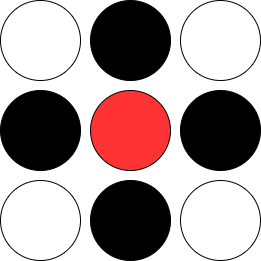
\includegraphics[width=0.5\textwidth, angle=0]{./fig/diagrams/neumann.png}
			\caption{von Neumann}
			\label{fig:neumann_neighbourhood}
		\end{subfigure}
    	&
		\begin{subfigure}[b]{0.3\textwidth}
			\centering
			
\includegraphics[width=0.5\textwidth, angle=0]{./fig/diagrams/moore.png}
			\caption{Moore}
			\label{fig:moore_neighbourhood}
		\end{subfigure}
    \end{tabular}
	\caption{Common neighbourhoods in discrete 2D environments of Agent-Based Simulation.}
	\label{fig:abs_neighbourhoods}
\end{center}
\end{figure}

\subsubsection{Implementation}
We start by defining our discrete 2D environment for which we use an indexed two dimensional array. In each cell the agents will store their current state, thus we use the \textit{SIRState} as type for our array data:

\begin{minted}[fontsize=\footnotesize]{haskell}
type Disc2dCoord = (Int, Int)
type SIREnv      = Array Disc2dCoord SIRState
\end{minted}

Next we redefine our monad stack and agent signal function. We use a StateT transformer on top of our Random Monad from step 4 with the previously defined SIREnv as type for the state. Our agent signal function now has only unit input and output type as we removed the data-flow mechanism for reasons of clarity. This also indicates through the types that the actions of the agents are only visible in side-effects through the monad stack they are running in.

\begin{minted}[fontsize=\footnotesize]{haskell}
type SIRMonad g = StateT SIREnv (Rand g)
type SIRAgent g = SF (SIRMonad g) () ()
\end{minted}

Instead of having a unique agent id an agent is now initialised through its coordinates in the environment and its initial state. 

\begin{minted}[fontsize=\footnotesize]{haskell}
sirAgent :: RandomGen g => Disc2dCoord -> SIRState -> SIRAgent g
sirAgent c Susceptible = susceptibleAgent c
sirAgent c Infected    = infectedAgent c
sirAgent _ Recovered   = recoveredAgent
\end{minted}

Again the recovered agent behaviour is the shortest one:
\begin{minted}[fontsize=\footnotesize]{haskell}
recoveredAgent :: RandomGen g => SIRAgent g
recoveredAgent = arr (const ())
\end{minted}

The implementation of a susceptible agent is now a bit different and a mix between previous steps. Instead of using data-flows the agent directly queries the environment for its neighbours and randomly selects one of them. The remaining behaviour is similar:

\begin{minted}[fontsize=\footnotesize]{haskell}
susceptibleAgent :: RandomGen g => Disc2dCoord -> SIRAgent g
susceptibleAgent coord = switch susceptible (const (infectedAgent coord))
  where
    susceptible :: RandomGen g => SF (SIRMonad g) () ((), Event ())
    susceptible = proc _ -> do
      makeContact <- occasionallyM (1 / contactRate) () -< ()
      if not (isEvent makeContact)
        then returnA -< ((), NoEvent)
        else (do
          e <- arrM_ (lift get) -< ()
          let ns = neighbours e coord agentGridSize moore
          s <- drawRandomElemS -< ns
          if Infected /= s
            then returnA -< ((), NoEvent)
            else (do
              infected <- arrM_ (lift $ lift $ randomBoolM infectivity) -< ()
              if infected 
                then (do
                  arrM (put . changeCell coord Infected) -< e
                  returnA -< ((), Event ()))
                else returnA -< ((), NoEvent)))
\end{minted}

Querying the neighbourhood is done using the \textit{neighbours} function. It takes the environment, the coordinate for which to query the neighbours for, the dimensions of the 2D grid and the neighbourhood information and returns the data of all neighbours it could find. Note that on the edge of the environment, it could be the case that fewer neighbours than provided in the neighbourhood information will be found due to clipping.

\begin{minted}[fontsize=\footnotesize]{haskell}
neighbours :: SIREnv -> Disc2dCoord -> Disc2dCoord -> [Disc2dCoord] -> [SIRState]
neighbours e (x, y) (dx, dy) n = map (e !) nCoords'
  where
    nCoords  = map (\ (x', y') -> (x + x', y + y')) n
    nCoords' = filter (\ (x, y) -> x >= 0 && y >= 0 && 
                                   x <= (dx - 1) && y <= (dy - 1)) nCoords
                           
neumann :: [Disc2dCoord]
neumann = [ top, left, right, bottom ]

moore :: [Disc2dCoord]
moore = [ topLeft,    top,    topRight,
          left,               right,
          bottomLeft, bottom, bottomRight ]

topLeft :: Disc2dCoord
topLeft  = (-1, -1)
top      = ( 0, -1)
topRight = ( 1, -1)
...
\end{minted}

The behaviour of an infected agent is nearly the same with the difference that upon recovery the infected agent updates its state in the environment from Infected to Recovered.

\begin{minted}[fontsize=\footnotesize]{haskell}
infectedAgent :: RandomGen g => Disc2dCoord -> SIRAgent g
infectedAgent coord = switch infected (const recoveredAgent)
  where
    infected :: RandomGen g => SF (SIRMonad g) () ((), Event ())
    infected = proc _ -> do
      recovered <- occasionallyM illnessDuration () -< ()
      if isEvent recovered
        then (do
          e <- arrM (\_ -> lift get) -< ()
          arrM (\e -> put (changeCell coord Recovered e)) -< e
          returnA -< ((), Event ()))
        else returnA -< ((), NoEvent)
\end{minted}

Running the simulation is now slightly different as we have an initial environment and also need to peel away the StateT transformer:
\begin{minted}[fontsize=\footnotesize]{haskell}
runSimulation :: RandomGen g => g -> Time -> DTime -> SIREnv -> [(Disc2dCoord, SIRState)] -> [SIREnv]
runSimulation g t dt e as = evalRand esRand g
  where
    steps    = floor (t / dt)
    dts      = replicate steps ()
    sfs      = map (uncurry sirAgent) as
    esReader = embed (stepSimulation sfs) dts
    esState  = runReaderT esReader dt
    esRand   = evalStateT esState e
\end{minted}

As initial state we use the initial environment and instead of returning agent states we simply return a list of environments, one for each step. The agent states can then be extracted from each environment.

Due to the different approach of returning the SIREnv in every step, we implemented our own MSF:
\begin{minted}[fontsize=\footnotesize]{haskell}
stepSimulation :: RandomGen g => [SIRAgent g]-> SF (SIRMonad g) () SIREnv
stepSimulation sfs = MSF (\_ -> do
  res <- mapM (`unMSF` ()) sfs
  let sfs' = fmap snd res
  e <- get
  let ct = stepSimulation sfs'
  return (e, ct))
\end{minted}

\subsubsection{Results}
We implemented rendering of the environments using the gloss library which allows us to cycle arbitrarily through the steps and inspect the spreading of the disease over time visually as in Figure \ref{fig:sir_env}.

\begin{figure}
\begin{center}
	\begin{tabular}{c c}
		\begin{subfigure}[b]{0.3\textwidth}
			\centering
			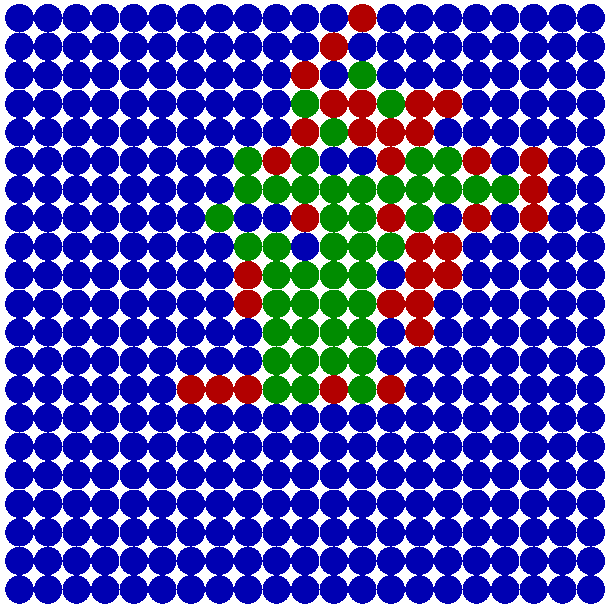
\includegraphics[width=1\textwidth, angle=0]{./fig/step5_environment/SIR_environment_30x30agents_t50_01dt.png}
			\caption{$t = 50$}
			\label{fig:sir_env_t50}
		\end{subfigure}
    	&
		\begin{subfigure}[b]{0.3\textwidth}
			\centering
			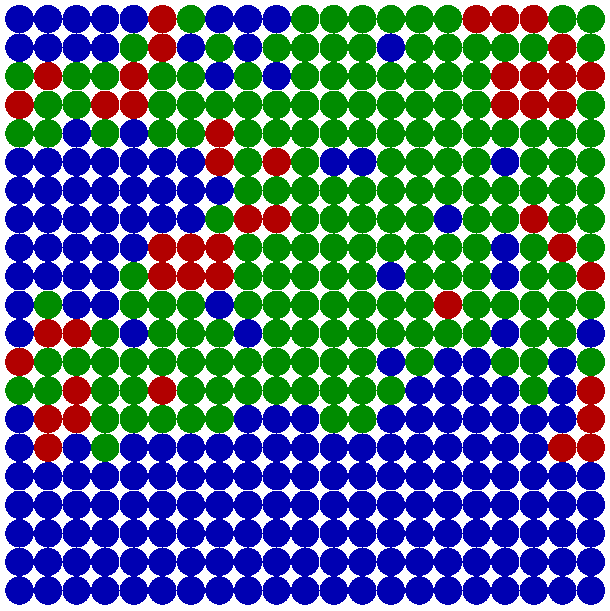
\includegraphics[width=1\textwidth, angle=0]{./fig/step5_environment/SIR_environment_30x30agents_t100_01dt.png}
			\caption{$t = 100$}
			\label{fig:sir_env_t100}
		\end{subfigure}
    	
    	\\
    	
		\begin{subfigure}[b]{0.3\textwidth}
			\centering
			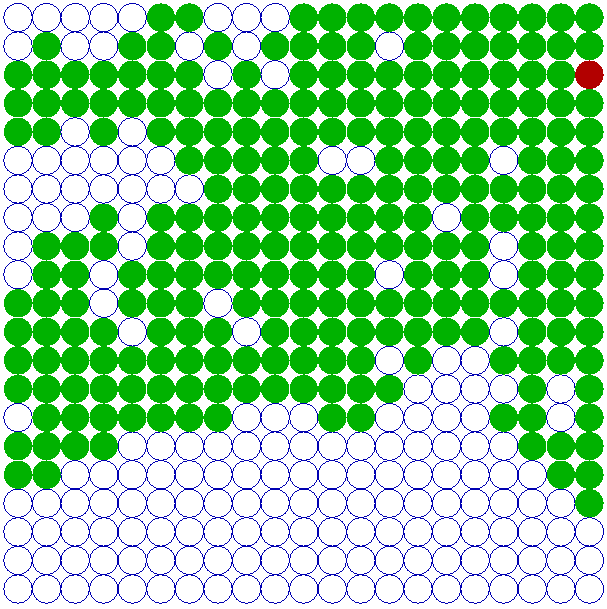
\includegraphics[width=1\textwidth, angle=0]{./fig/step5_environment/SIR_environment_30x30agents_t160_01dt.png}
			\caption{$t = 160$}
			\label{fig:sir_env_t160}
		\end{subfigure}
		& 
		\begin{subfigure}[b]{0.38\textwidth}
			\centering
			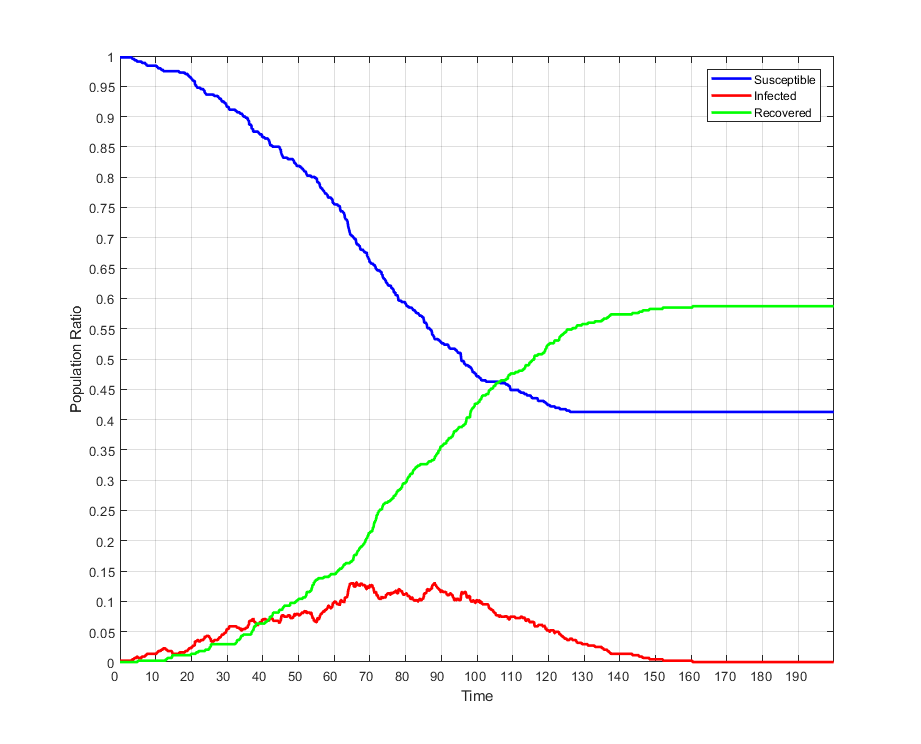
\includegraphics[width=1\textwidth, angle=0]{./fig/step5_environment/SIR_dynamics_30x30agents_300t_01dt.png}
			\caption{Dynamics over time}
			\label{fig:sir_dynamics_30x30agents_300t_01dt}
		\end{subfigure}
	\end{tabular}
	
	\caption{Simulating the agent-based SIR model on a 21x21 2D grid with Moore neighbourhood and a single infected agent at the center and same SIR parameters. Simulation run until $t = 200$ with fixed $\Delta t = 0.1$. Last infected agent recovers shortly after $t = 160$. The susceptible agents are rendered as blue hollow circles for better contrast.}
	\label{fig:sir_env}
\end{center}
\end{figure}

Note that the dynamics of the spatial SIR simulation which are seen in Figure \ref{fig:sir_dynamics_30x30agents_300t_01dt} look quite different from the SD dynamics of Figure \ref{fig:sir_sd_dynamics}. This is due to a much more restricted neighbourhood which results in far fewer infected agents at a time and a lower number of recovered agents at the end of the epidemic, meaning that fewer agents got infected overall.

\subsubsection{Discussion}
At first the environment approach might seem a bit overcomplicated and one might ask what we have gained by using an unrestricted neighbourhood where all agents can contact all others. The real win is that we can introduce arbitrary restrictions on the neighbourhood as shown using the Moore neighbourhood. Of course the environment is not restricted to a discrete 2D grid and can be anything from a continuous N-dimensional space to a complex network - one only needs to change the type of the StateT monad and provide corresponding neighbourhood querying functions. The ability to place the heterogeneous agents in a generic environment is also the fundamental advantage of an agent-based over the SD approach and allows to simulate much more realistic scenarios. Note that for reasons of clarity we have removed the data-flow approach from this implementation which results in the unit-types of input and output. In a full blown agent-based simulation library we would combine both approaches.

Generally, there exist four different environment scenarios in an agent-based model
\begin{enumerate}
	\item Passive read-only - implemented in the previous steps, where the environment does never change and is passed as static information, e.g. list of neighbours, to each agent.
	\item Passive read/write - implemented in this step. The environment itself is not modelled as an active process but just as shared data which can be accessed and manipulated by the agents.
	\item Active  read-only - can be implemented by adding an environment agent which broadcasts changes in the environment to all agents using the data-flow mechanism.
	\item Active read/write - can be implemented as in this step plus adding an environment agent which reads/writes the environment e.g. regrowing some resources.
\end{enumerate}

Attempting to introduce an active/passive read/write environment to the Yampa implementation would be quite cumbersome. A possible solution could be to add a type-parameter \textit{e} which captures the type of the environment and then pass it in through the input and allow it to be returned in the output of an agent signal function. We would then end up with $n$ copies of the environment - one for each agent - which we need to fold back into a single environment. Having an active environment complicates things even further. All these problems are not an issue when using MSFs with a StateT which is a compelling example for making the transition to the more general MSFs. The convenient thing is that although conceptually all agents act at the same time, technically by using \textit{mapM} in stepSimulation they are run after another which also serialises the environment access which gives every agent exclusive read/write access while it is active.

%In the last step we will introduce synchronised agent-transaction as the final agent-agent interaction mechanism. This is a quite sophisticated concept: synchronised agent-transactions which allow an arbitrary number of interactions between two agents without time lag. The use-case for this are price negotiations between multiple agents where the agents need to come to an agreement in the same time-step as described in TODO cite sugarscape.